\clearpage
\section{Temporary diagnostic: signal versus filename length}\label{sec:temporary-length}
For this exploratory test only, suppose the heterodyne phase were proportional to the length $L$ in each TG filename, $\psi(L)=\beta L+\psi_0$. If all other quantities were identical, tutorial Eq.~(4.6) would then predict, at a fixed delay $t_*$,
\begin{equation}
S(L,t_*)=P(t_*)+G(t_*)\cos(\beta L+\psi_0).
\end{equation}
Figure~\ref{fig:temporary-length} plots the actual first-repeat signal at the common recorded delay $t_*=\SI{5}{ps}$ from each of the four TG files. This delay is present exactly in every file, so no interpolation is used. The retained-repeat mean and its standard error are included to show repeat variability. No baseline subtraction or normalization is applied. Delay-calibration and nominal-length uncertainties, and uncertainties of individual recorded points, are unavailable. The PP file has no grating-length label and is not assigned an artificial horizontal coordinate.

\begin{figure}[!htbp]
\centering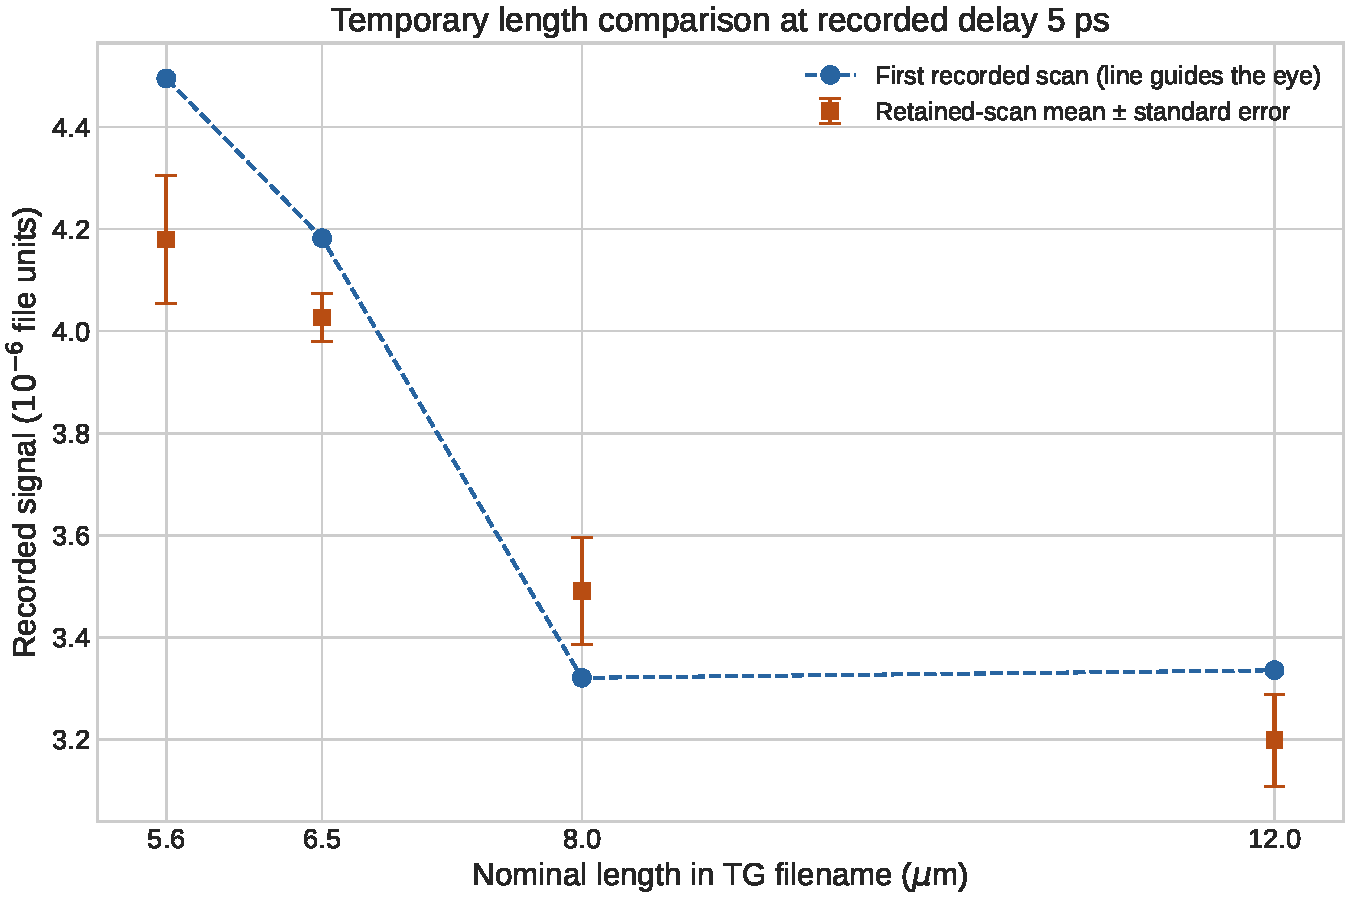
\includegraphics[width=\linewidth]{../plots/temporary_length_snapshot.pdf}
\caption{Temporary fixed-delay snapshot for the hypothesized length-to-phase relation. Blue circles are values from the first recorded repeat at \SI{5}{ps}; the dashed segments only connect these points and are not a cosine fit. Orange squares show means over the scans retained by the report's existing screening procedure; error bars are one standard error across retained scans. The horizontal values are the nominal filename lengths, not the demagnified sample periods or calibrated phases. Individual-point and calibration uncertainties are unquantified.}\label{fig:temporary-length}
\end{figure}
\FloatBarrier

The first-repeat values show an overall decrease, with a small rise between the last two points; the retained-repeat means decrease throughout. This snapshot does not establish an oscillation: a decreasing segment could be consistent with part of a cosine, but four points without a phase calibration cannot identify a fringe period reliably. No sinusoidal fit or phase proportionality constant is inferred.

The experimental interpretation remains that the filename lengths specify phase-mask \emph{periods}, with $\Lambda_{\rm sample}=L/4$. Changing $L$ therefore changes $q$ and the grating dynamics, whereas the phase scan in tutorial Fig.~4.6 varies the local-oscillator phase at a fixed grating period. The present graph tests the proposed visual comparison but does not reproduce that controlled phase scan. This section is temporary and is not used in the reported parameter estimates.
